In this section we break down the implementation of the system into its core components, following the methodology and requirements outlined in the previous sections. The full code is attached in the \ref{Appendix} appendix.

The goal was to create a system which not only fixes bugs but is also portable /deployable across different repositories and configurable to some extend.

The resulting system consists of two main components. The \textbf{APR core} which hold the core logic for the repair process and lives inside a docker image, making it portable and easy to deploy. The second component is the \textbf{Continuous Integration Pipeline} which integrates the core logic within a GitHub repository. It serves as the entry point and orchestrates the execution of the APR core based on issues and configured triggers in the repository.

\section{System Components}

\textbf{APR Core:}

The APR core contains the main bug fixing logic, its written in python. Embedding it into a Docker Image \footnote{link to docker} it remains easily portable and small in memory footprint. In order to use the APR core the following environment needs to passed to the container:

\renewcommand{\arraystretch}{1.5} % Set row spacing to 1.5
\begin{longtable}{@{\extracolsep{\fill}} p{4cm} | p{6cm} | p{4cm}  @{}}
    \caption{Container Inputs} \label{tab:container-inputs}                                                     \\

    \toprule
    \textbf{Name}      & \textbf{Description}                                            & \textbf{Type}        \\
    \midrule
    \endfirsthead

    \bottomrule
    \endfoot
    git repository     & files where APR should look for fixes                           & docker volume mount
    \\ \hline
    GITHUB\_TOKEN      & GitHub token for authentication and API access                  & environment variable \\
    \hline
    LLM\_API\_KEY      & API key for the LLM provider to generate fixes                  & environment variable \\
    \hline
    ISSUE\_TO\_PROCESS & The issue to process, can be a single issue or a list of issues & environment variable \\
    \hline
    GITHUB\_REPO       & The GitHub repository where the issues are located              & environment variable \\
    \hline
\end{longtable}

With this environment set the APR core iterates over all issues which are fetched from the (ISSUE TO PROCESS) environment variable. For each issue the main APR logic is executed. This main logic is a predefined flow which is made up of the implemented stages and tools.

At first the workspace (branch checkout) and the issue repair context is set up. The context is the main data structure for the issue repair and is processed at every step.

\begin{lstlisting}[caption={Context JSON}]
context = {
        "bug": issue,
        "cfg": cfg,
        "state": {
            "current_stage": None,
            "current_attempt": 0,
            "branch": None,
            "repair_successful": False,
        },
        "files": {
            "source_files": [],
            "fixed_files": [],
            "diff_file": None,
            "log_dir": str(log_dir),
        },
        "stages": {},
        "attempts": [],
        "metrics": {
            "github_run_id": os.getenv("GITHUB_RUN_ID"),
            "issue_number": issue["number"],
            "issue_title": issue["title"],
            "execution_repair_stages": {},
            "repair_successful": False,
            "attempts": 1,
        },
    }
\end{lstlisting}

%TODO add system instruction
A stage uses the context to perform a specific task in the bug fixing process and returns the context with its added context. The implemented stages are Localize, Fix, Build and Test. The repair process starts with the localization stage. This stage localizes the files needed to fix the bug in the codebase using the configured LLM Model via the providers SDK/API. The prompt is build using the issue and a constructed hierarchy of the repositories file structure. The response is expected to return a list of files where the bug might be located.

\begin{lstlisting}[caption={Localization Prompt}]
system_instruction = "You are a bug localization system. Look at the issue description and return ONLY the exact file paths that need to be modified."

prompt = f"""
    Given the following GitHub issue and repository structure, identify the file(s) that need to be modified to fix the issue.

    Issue #{issue['number']}: {issue['title']}
    Description: {issue.get('body', 'No description provided')}

    Repository files:
    {json.dumps(repo_files, indent=2)}

    Return a JSON array containing ONLY the paths of files that need to be modified to fix this issue.
    Example: ["path/to/file1.py", "path/to/file2.py"]
    """
\end{lstlisting}

%TODO add system instruction
With the localized files in the context the Fix stages comes next. Again this stage makes use of the configured LLM API to fix the localized files. A prompt contains the issue and file names with file content. The response is expected to contain a list of edits for each file while also allowing the LLM to specify that no changes need to be made in a file. The generated edits are then applied to the files in the workspace. The context is updated with the new file content.

\begin{lstlisting}[caption={Repair Prompt}]
system_instruction = "You are part of an automated bug-fixing system. Please return the complete, corrected raw source files for each file that needs changes, never use any markdown formatting. Follow the exact format requested."

base_prompt = f"""
    The following Python code files have a bug. Please fix the bug across all files as needed.

    {files_text}

    Please provide the complete, corrected source files. If a file doesn't need changes, you can indicate that.
    For each file that needs changes, provide the complete corrected file content.
    Format your response as:

    === File: [filepath] ===
    [complete file content or "NO CHANGES NEEDED"]

    === File: [filepath] ===
    [complete file content or "NO CHANGES NEEDED"]
    """
    
\end{lstlisting}

For validation 2 stages are available Build and Test. The Build stage is responsible for validating syntactics of the changes made in the Fix stage. It checks if the code can be built successfully. For python this means checking if the syntax is correct and follows standardized code quality rules \footnote{todo}. This is archived by first formatting the code using the Python formatter Black\footnote{todo} followed by linting using flake8\footnote{todo}.

If a test command is configured the Test stage is executed next. This stage runs the tests defined in the repository using the configured test command.

In case Build or Test fail, the context is updated with the error messages, and the system will retry the Fix stage with a new attempt. For attempts additional feedback is generated using the previous code and stage results with details.

When maximum number of attempts is reached and the code does not pass validation  unsuccessful repair is reported to the issue by creating a comment using the Github API.

On successful Build and Test the issue is marked as a successfully repaired. The file changes are committed and a diff file is generated. The branch is pushed to the remote repository, and a pull request is created. The pull request contains the changes made in the Fix stage, and the issue is linked to the pull request.

During execution the APR core logs its actions, which can be used for debugging and provides transparency about the repair process. Furthermore it collects metrics such as the number of attempts, execution times, and token usage, which are essential for analyzing the effectiveness and performance of the APR system.

The agent core is designed to be modular and extensible, allowing for future enhancements and additional stages or tools to be integrated as needed. It is also designed to be lightweight, ensuring that it can run efficiently within a CI/CD environment.

\begin{figure}[H]
    \centering
    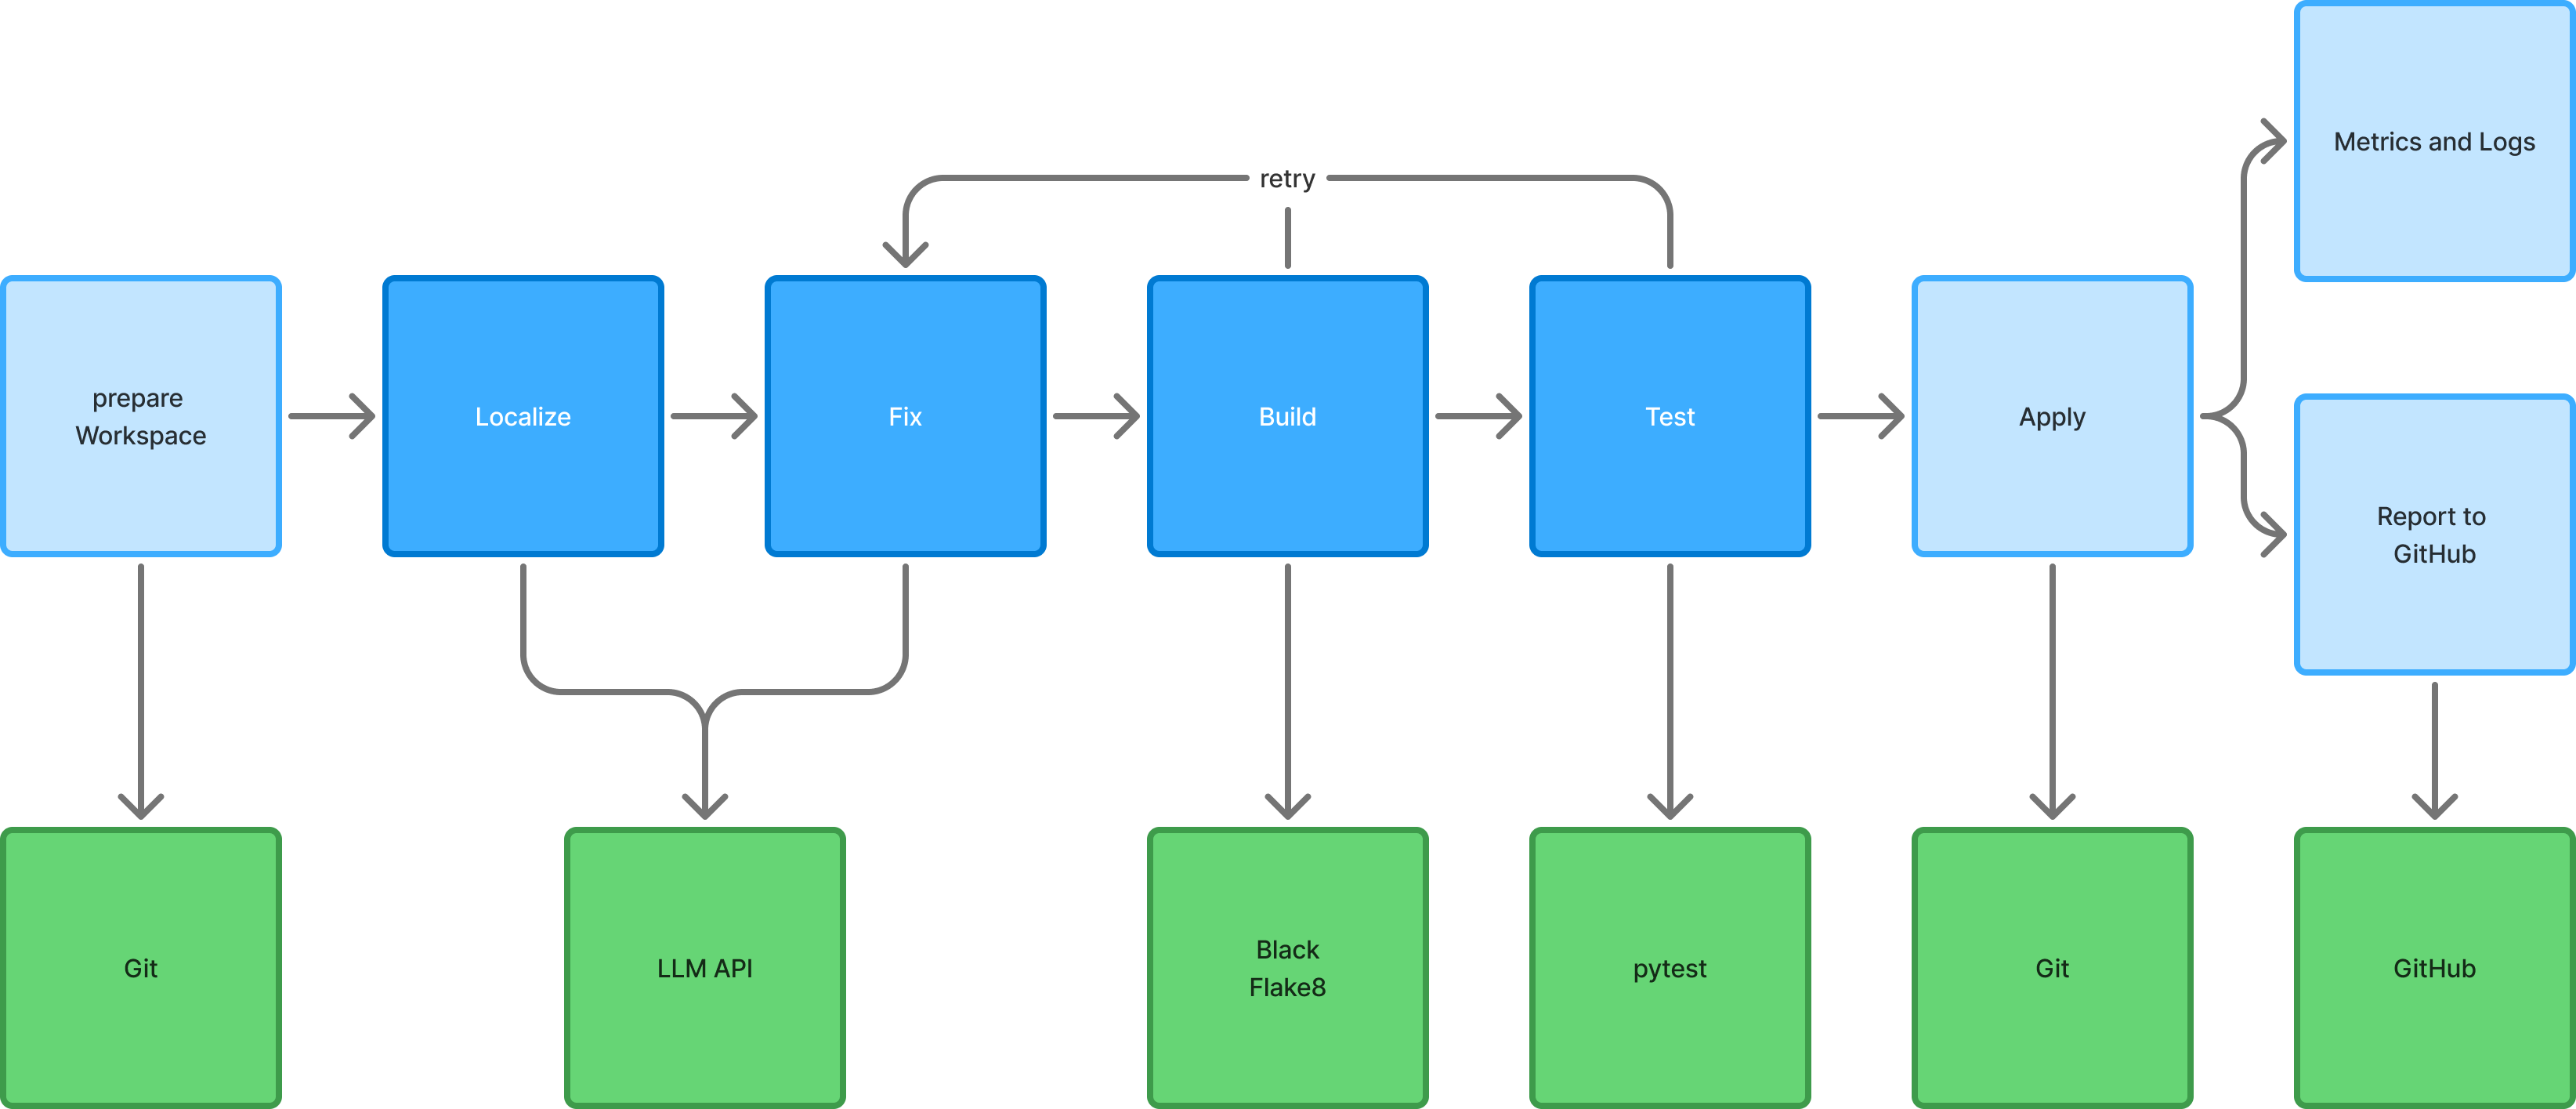
\includegraphics[width=1\textwidth]{images/flowcharts/apr-core.png}
    \caption{APR Core Logic}
    \label{fig:apr-core}
\end{figure}

\textbf{Continuous Integration Pipeline:}

The Github Action Workflow integrates the APR core into the desired GitHub repository. It is written in YAML\footnote{todo} according to the Github Action standard. %\ref{} 
We will use runners provided and hosted by Github which takes away the overhead of managing our own runners but comes at the cost of unknown performance and availability. %\cite{}
The Workflow is made up of multiple triggers and jobs. Triggers work by using events happening in the GitHub repository and serve as the entry point for executing the jobs. Given the triggers the workflow can is executed two different ways:

\begin{itemize}
    \item Process all issues with desired state for repair. Triggered by manual dispatch (``workflow\_dispatch'') or scheduled execution (``cron'').
    \item Process a single issue. Issue is labeled with the configured labels (``issue\_labeld'') or when extra information is added or edited on an issue in form of a comment (``issue\_comment'').
\end{itemize}

The trigger event information gets passed as environment variables to the first job. ``gate'' uses this data to evaluating if the issue should be processed or skipped using a python script (filter\_issues.py). This script checks the labels and resolves the issue state to determine if the issue is relevant for the APR process. If no issues pass this ``gate'' the job ``skipped'' is executed, which simply logs that no issues were found to process and exits the workflow. When issues pass the ``gate'' the ``bugfix'' job is started.  This job is responsible for executing the APR core logic. It provides necessary prerequisites for the APR core Docker container to run \ref{tab:container-inputs} and perform the repair. This includes checking out and mounting the repository, setting up environment variables, and providing the necessary permissions for the core to edit repository content, create pull requests, and write issues.

For giving access to the agent cores logs and metrics the job provides the logs directory as an artifact which is available after the workflow run is completed.

\begin{figure}[H]
    \centering
    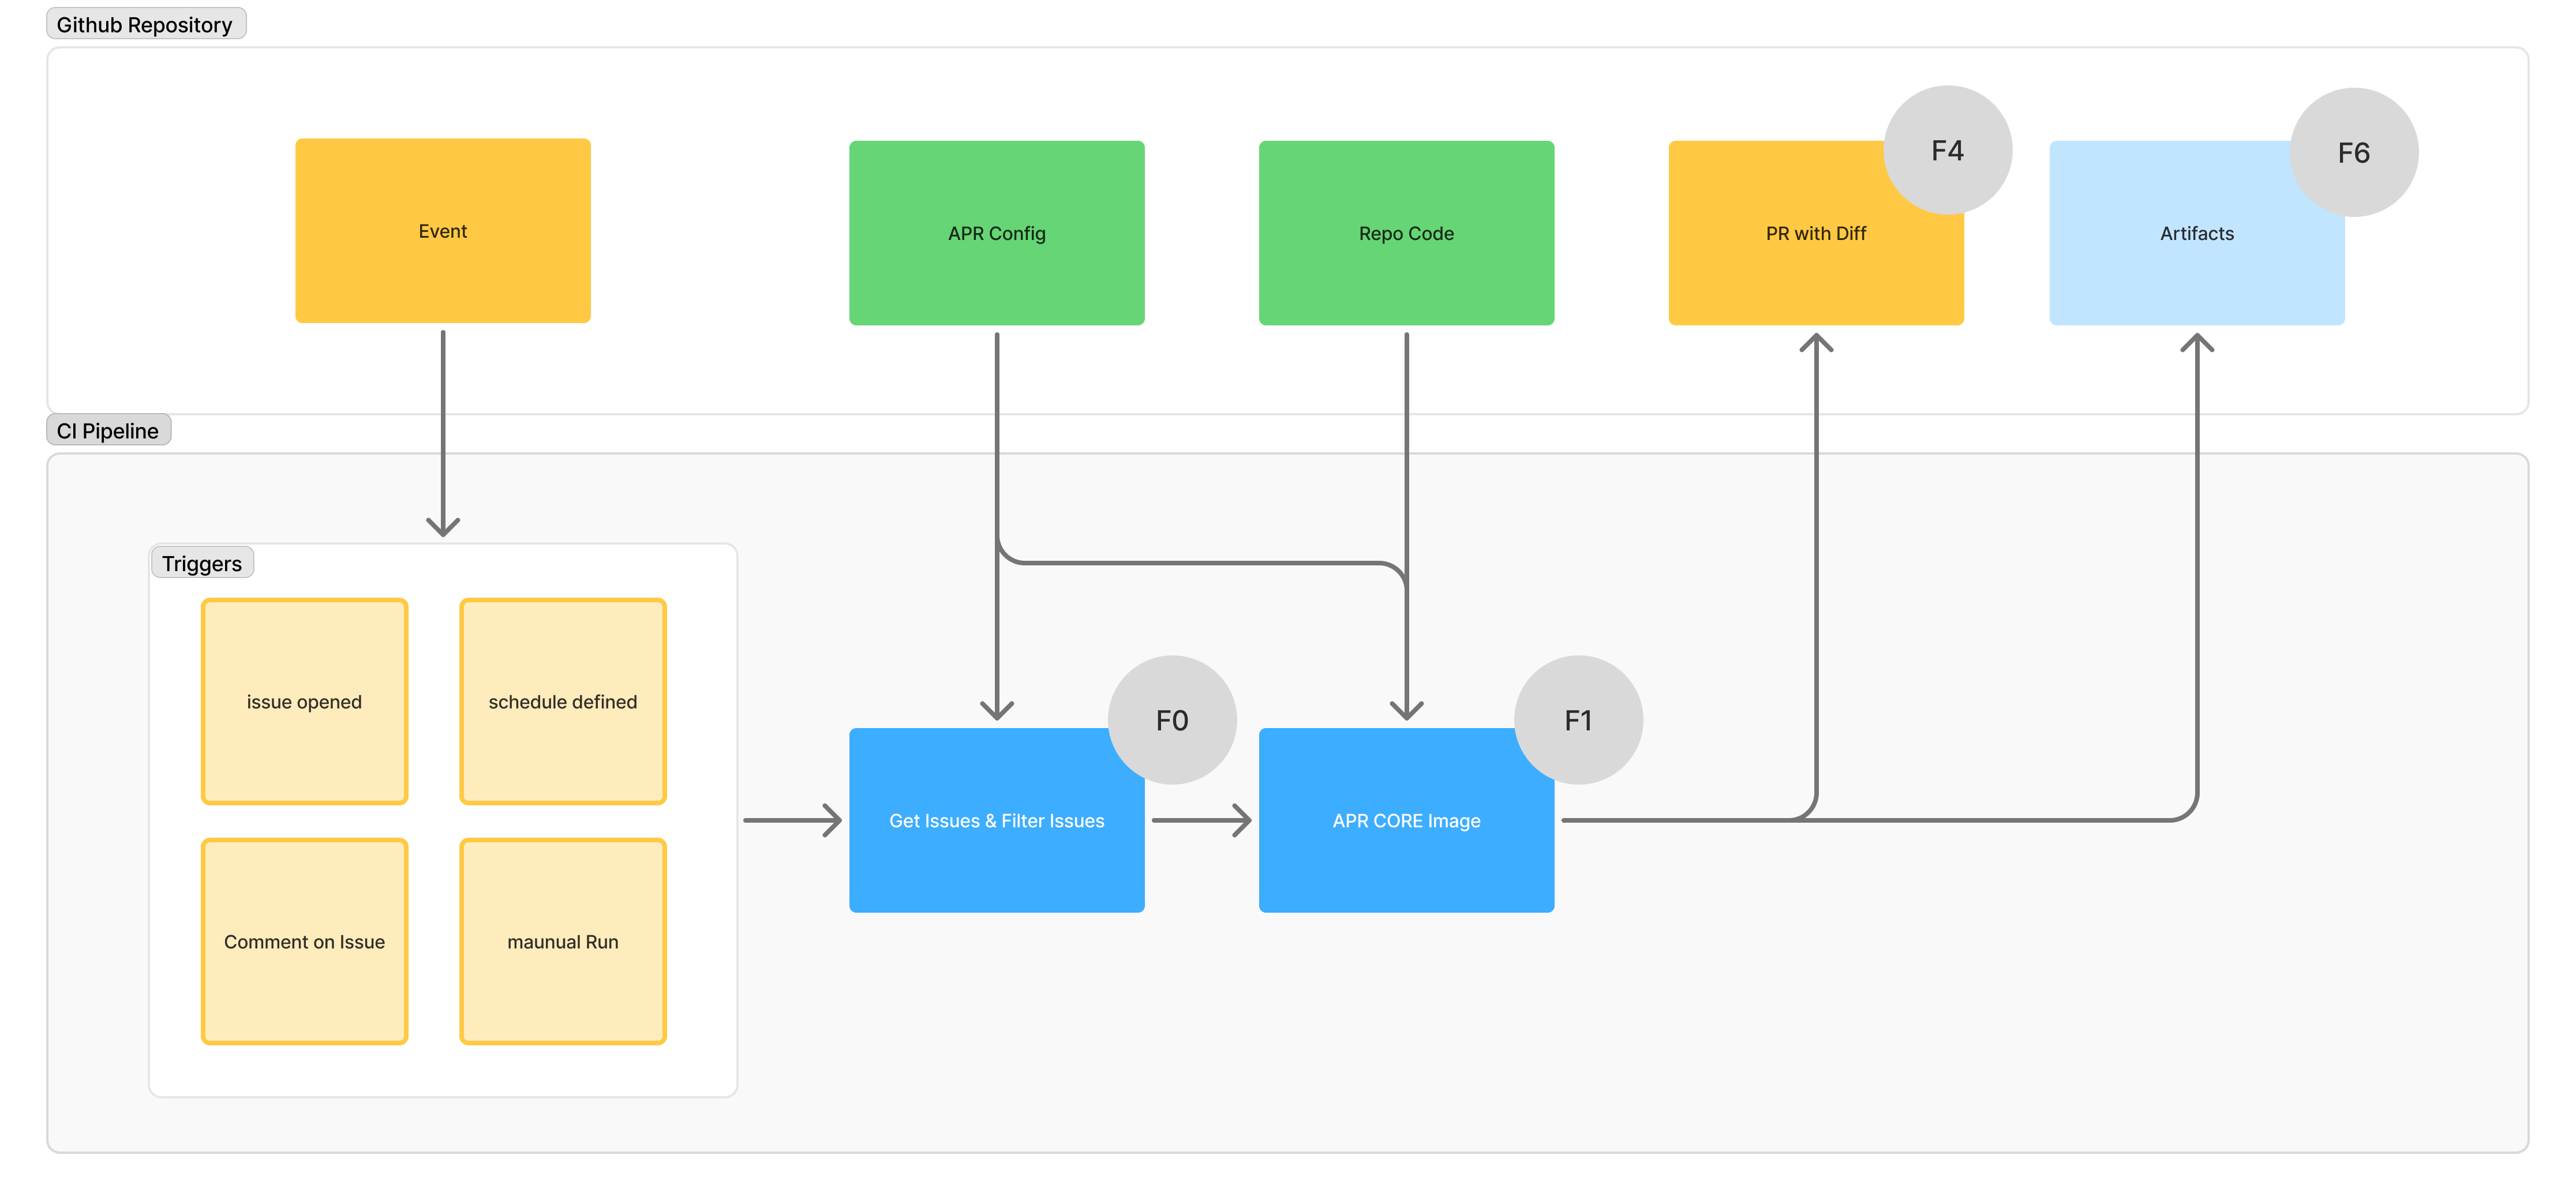
\includegraphics[width=1\textwidth]{images/flowcharts/ci.png}
    \caption{APR Core Logic}
    \label{fig:ci}
\end{figure}

To use this workflow in a repository, it needs to be placed in the `.github/workflows` directory of the repository along with the `filter\_issues.py` in `.github/scripts`.
The following adjustments need to be made to the repository:
\begin{itemize}
    \item Add Secrets: LLM provider API key, GITHUB TOKEN
    \item enable GitHub actions permission to create pull requests in repo settings
\end{itemize}


\section{System Configuration}

To fulfill requirement X some of the systems behavior can be controlled by adjusting a configuration. A configuration is optional when no configuration is in place the system will use default configuration which is defined in the code. The configuration is written in YAML and can be placed at the root of the repository. This allows for easy customization of the system without changing the code itself. The configuration file is named 'bugfix.yml' and is read by the APR core and CI Pipeline during execution. The configuration allows for controlling labels, workdir, branches, attempts and LLM models used for the repair process.

\renewcommand{\arraystretch}{1.5}
\begin{longtable}{@{\extracolsep{\fill}} p{3.5cm} | p{11cm} @{}}
    \caption{Configuration Fields and Descriptions} \label{table:configuration}                                                         \\
    \toprule
    \textbf{Configuration Field} & \textbf{Description}                                                                                 \\
    \midrule
    \endfirsthead

    \bottomrule
    \endfoot

    to\_fix\_label               & The label used to identify issues that need fixing.                                                  \\ \hline
    submitted\_fix\_label        & The label applied to issues when a fix is submitted.                                                 \\ \hline
    failed\_fix\_label           & The label applied to issues when a fix fails.                                                        \\ \hline
    workdir                      & The working directory where the code resides, used for mounting in the Docker container.             \\ \hline
    test\_cmd                    & The command used to run tests on the codebase.                                                       \\ \hline
    branch\_prefix               & The prefix for branches created for bug fixes, allowing for easy identification of bug fix branches. \\ \hline
    main\_branch                 & The main branch of the repository where bug fix branches are based.                                  \\ \hline
    max\_issues                  & The maximum number of issues to process in a single run.                                             \\\hline
    max\_attempts                & The maximum number of attempts to fix an issue before giving up.                                     \\ \hline
    provider                     & The LLM provider used for generating fixes.                                                          \\ \hline
    model                        & The specific model from the LLM provider used for generating fixes.                                  \\
\end{longtable}


The full implementation is listed in Appendix~\ref{Appendix}